\documentclass[a4paper,11pt]{article}
\usepackage{latexsym,amssymb,enumerate,amsmath,epsfig,amsthm}
\usepackage[margin=1in]{geometry}
\usepackage{setspace,color}
\usepackage{graphics}
\usepackage{subfigure}
\usepackage{hyperref}
\usepackage{subfiles} 
\usepackage{float}

\newcommand{\redcolor}[1]{\textcolor{red}{#1}}
\graphicspath{ {./images/} }



%\newcommand{\x}{\mathbf{x}}
%\newcommand{\y}{\mathbf{y}}
%\newcommand{\bv}{\mathbf{v}}
%\newcommand{\n}{\mathbf{n}}
%\newcommand{\colored}[1]{\textcolor{red}{#1}}
%\newtheorem{thm}{Theorem}[section]
%\newtheorem{prop}{Proposition}[section]
%\newtheorem{obser}{Observation}[section]
%\newtheorem{corollary}{Corollary}[section]

%\doublespacing

\title{Blind Source Separation of Stereo Mixtures Using Wavelet Transform}
\author{
CHOI, Seung-ryeol \thanks{Department of Mathematics, the Hong Kong University of Science and Technology, Clear Water Bay, Hong Kong. Email: {\bf schoiak@connect.ust.hk}}
\and
KIM, Minji \thanks{Department of Mathematics, the Hong Kong University of Science and Technology, Clear Water Bay, Hong Kong. Email: {\bf mkimao@connect.ust.hk}}  
}

\markboth{First author}{MATH4992 Project Final Report}
\pagestyle{myheadings}
\date{30 November 2022}

\begin{document}
\thispagestyle{plain}
\maketitle


\begin{abstract}
Blind Source Separation refers to a problem where the independent sources should be separated from the set of measurements without or with little information about the sources or the mixing process. It is often challenging when the situation is underdetermined i.e. the number of sources is more than the number of measurements. In this project, we will investigate an approach for solving the Blind Source Separation Problem with the assumption that the source signals have sparse approximation supports.
\end{abstract}

\section{Introduction}

\subsection{Background}
Blind Source Separation problem is a well-known signal processing problem where the independent sources should be separated from the mixture of signals. An example is separating the sounds of K musical instruments from P microphones recordings without knowing the original sources and their mixing parameters.
\\ \\
\noindent A linear model is appropriate for representing a mixture of sound sources. The P channel measurement of K sources can be written as,

\begin{equation}
    y_p[n] = \sum \limits _{{k=1 }}^{K}{m_{p,k}}{s_k[n]} + \epsilon_k[n], \;for \;   1\leqslant{p}\leqslant{P} \;
\end{equation}

\noindent where $ M = \{m_{p,k}\}_{1\leq p \leq P, 1\leq k \leq K} $ is the mixing matrix and $\epsilon_k[n]$ are measurement noise.
\\

\noindent The number of K sources is unknown, and it is often greater than the number of measurements P which makes the problem underdetermined. Thus, knowing the mixing matrix M is not enough to recover the sources $s_k$ from the measurement $y_p$.
In this paper, we will introduce a successful method for source separation under the condition that sources have sparse approximation supports.


\subsection{Blind Source Separation}
Blind source separation is a fundamental of signal processing that has received a great amount of attention recently. Recently, many researchers have explored a number of techniques to solve the blind source separation problem\cite{1576973}\cite{ica}\cite{6025435}. One effective source separation method is based on stochastic models, where the sources must be independent\cite{COMON1994287}. However, it can be challenging to formulate a stochastic model of complicated signals and hence confirm their independence. \\
\\
\noindent Instead, we will use a method that is based on weaker deterministic models.
Jourjine, Rickard, and Yilmaz as well as Zibulevsky et al introduced an algorithm called Sparse Blind Source Separation, which estimates the mixing parameters under the assumption that the source supports do not overlap too much in an appropriate domain.\cite{1461442}\cite{BOFILL20012353}



\subsection{Project Objective}
In this paper, we aim to achieve two main project objectives:\\
\indent 1. Estimating the mixing matrix \textbf{\textit{M}} \\
\indent 2. Separating independent $\boldsymbol{S}$ sources from the measurements $\boldsymbol{y_p[n]}$. 



\section{Methodology}

\subsection{Multi-level Discrete Wavelet Transform}
For blind source separation, the mixing parameters $m_{p,k}$ can be estimated by defining a dictionary where different sources have a sparse representation. Here, we will use a Multi-level Discrete Wavelet Transform to obtain such a dictionary.\\
\\
Multi-level Discrete Wavelet Transform decomposes signals into a shifted and scaled versions of the basis wavelet. At different dilatation, wavelet coefficients can be obtained that represent various levels of frequencies. As we can observe from Figure 1, smaller scales i.e., lower-level wavelet transform, are associated with high frequencies, whereas larger scales are associated with the low-frequency information. Since high-frequency components are a complement to low-frequency components, wavelet coefficients then can be our dictionary that has a sparse representation.


\begin{figure}[H]
    \centering
    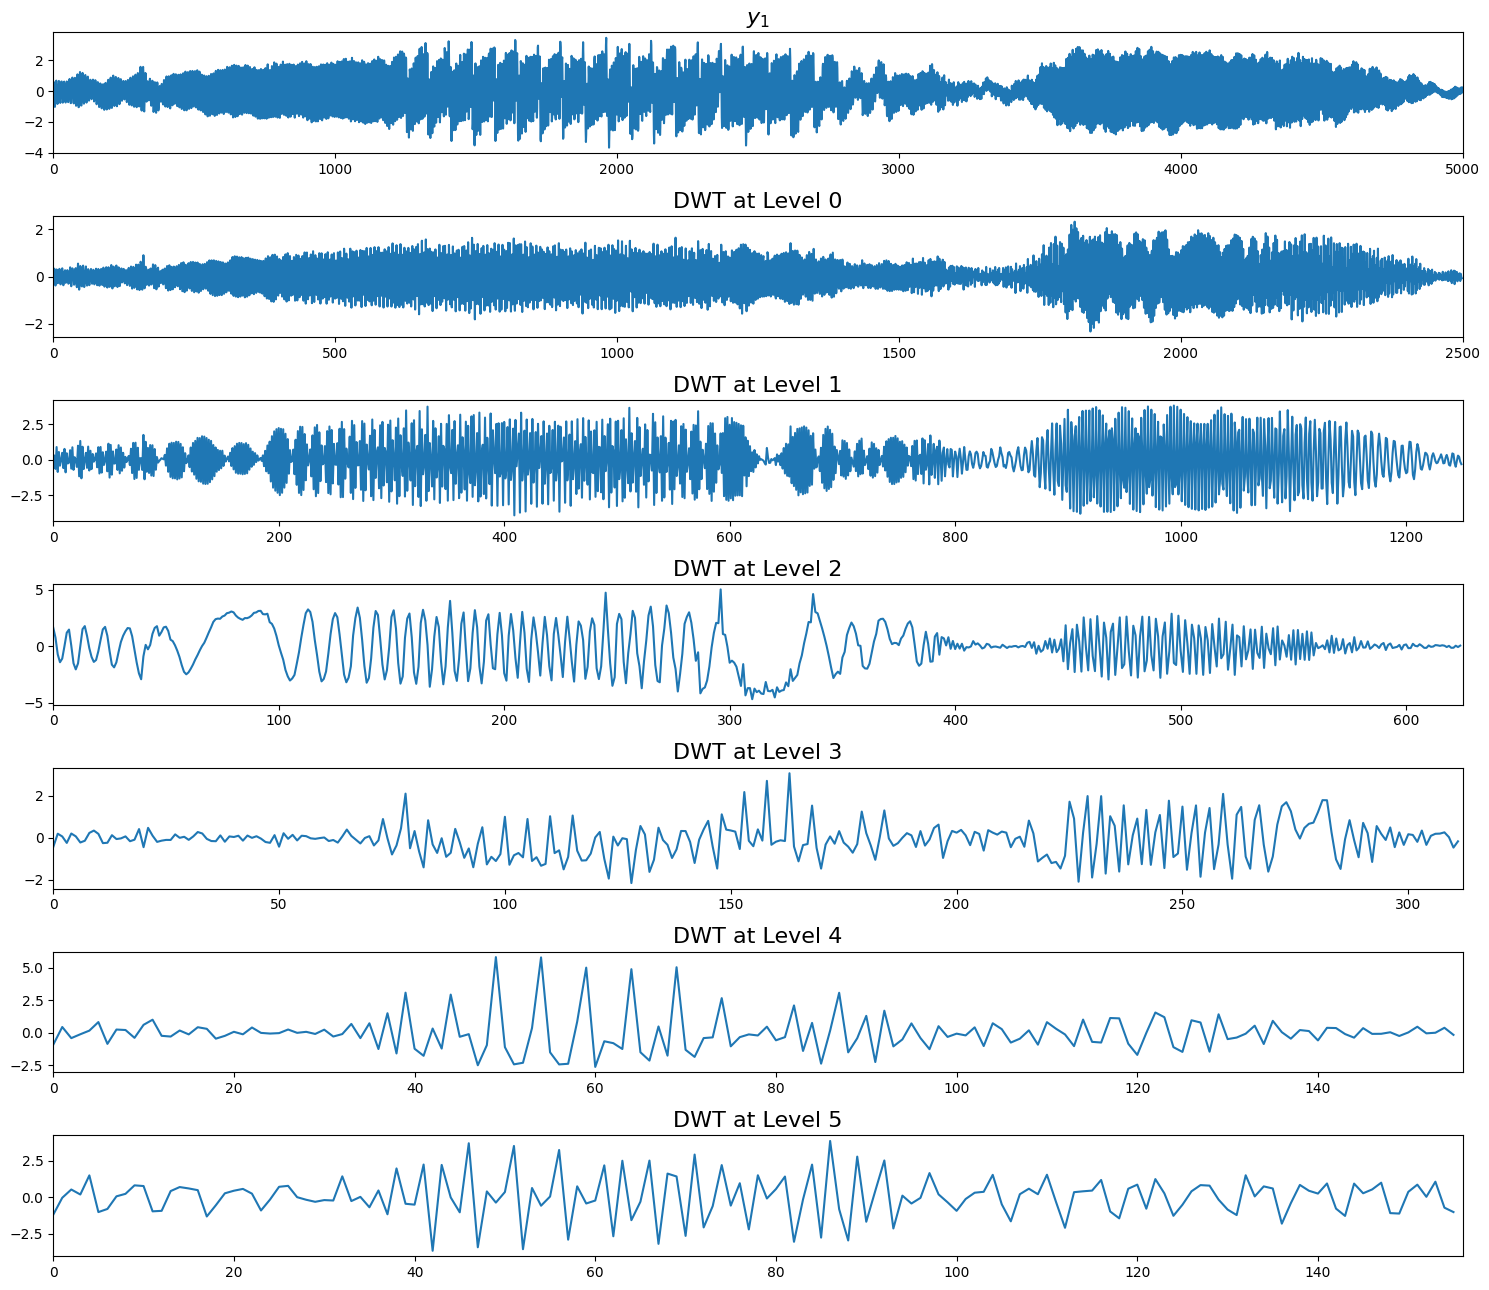
\includegraphics[width=0.65\linewidth]{sources/wt.png}
    \caption{\textbf{(a)} Multi-level Discrete Wavelet Transform of $y_1$}
    \label{fig:my_label}
\end{figure}



\subsection{Assumption}
Sparse blind source separation requires constrained condition i.e., the source supports directions are distinct. In order to fulfill the constrained condition, We assume that no two mixing directions are parallel such that,
\begin{equation}
\vec{m}_{\,a} \neq k\vec{m}_{\,b}, for \ some \ \vec{m}_a, \ \vec{m}_b \in M, a \neq b
\end{equation} 
where $k$ is some constant in $\mathbb{R}$.\\
\\
In addition, for the simplicity of the experiment formulation we assume that the noise term $\epsilon_p$ is negligible such that,
\begin{equation}
    \epsilon_p = 0, \quad \text{for} \; 1\leq p \leq P
\end{equation}
which makes our measurement equation $y_p[n]$ as below:
\begin{equation}
    y_p[n] = \sum \limits _{{k=1 }}^{K}{m_{p,k}}{s_k[n]}, \;for \;   1\leqslant{p}\leqslant{P} \;
\end{equation}


\subsection{Data Preprocessing}
Before we begin our experiment, we will simulate the stereo channel measurement of 3 sound sources which are the bird, male and female sounds accordingly. We will first construct a mixing matrix M, which will be the ground truth mixing parameters. The measurements $y_n$, then can be obtained by taking the inner product of the original sources and the mixing matrix.
To ensure the data uniformity, we used normalized sources.\\
\\
Since the source supports of $s_k[n]$ should have distinct directions we have set the mixing matrix using trigonometry in such a way that,
\begin{equation}
M = 
\begin{bmatrix}m_{1,1}&m_{1,2}&m_{1,3}\\
m_{2,1}&m_{2,2}&m_{2,3}
\end{bmatrix}
= \begin{bmatrix}\cos(\theta_1)&\cos(\theta_2)&\cos(\theta_3)\\
\sin(\theta_1)&\sin(\theta_2)&\sin(\theta_3)
\end{bmatrix}
\end{equation}
\[
\text{where} \quad
\theta_{k} \neq \theta_{k^{'}}\; \text{and} \; k \neq k^{'} \; \text{for} \;\; k, k^{'} \in \{1, 2, 3\}
\]
\\
Then we will take the inner product of the sources and the mixing matrix.
\begin{equation}
    Y = \binom{y_1[n]}{y_2[n]}  = \langle M, S \rangle
\end{equation}
In the other words, we obtained the measurements that are the linear combinations of the original source signals with mixing parameters $m_{p,k}$.

\begin{equation}
\begin{split}
    y_1[n] & = m_{1,1}s_1[n] + m_{1,2}s_2[n] +m_{1,3}s_3[n] \\
    y_2[n] & = m_{2,1}s_1[n] + m_{2,2}s_2[n] +m_{2,3}s_3[n]
\end{split}
\end{equation}
\\

\begin{figure}[H]
\centering
\subfigure[]{
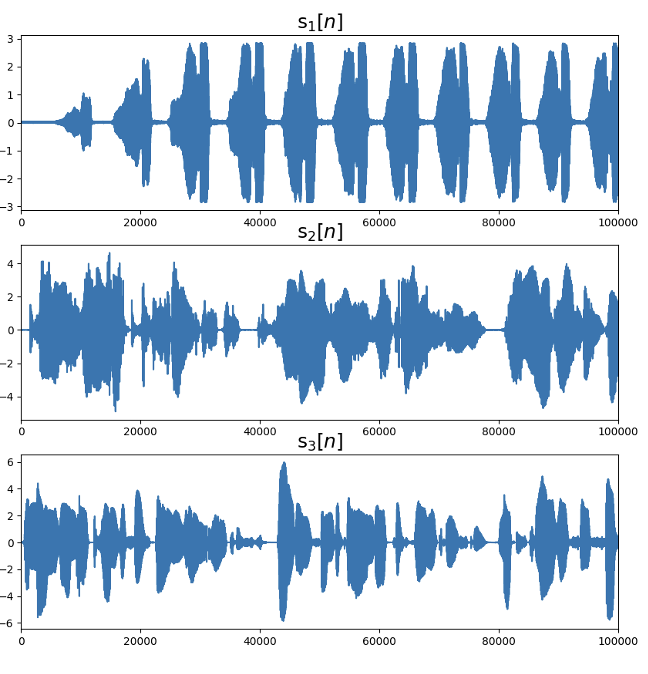
\includegraphics[width=0.35\linewidth]{sources/s.png}
}
\centering
\subfigure[]{
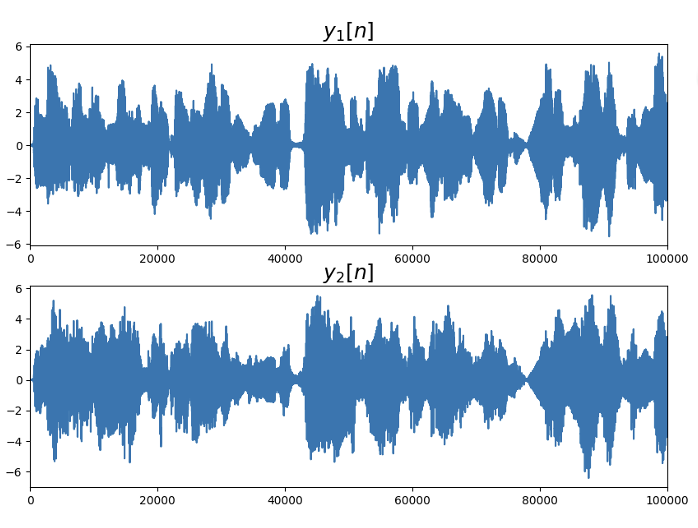
\includegraphics[width=0.35\linewidth]{sources/y.png}
}
\caption{\textbf{(a)} source signals $s_1[n]$, $s_2[n]$, and $s_3[n]$ \; \textbf{(b)} mixture of sources $y_1[n]$ and $y_2[n]$}
\label{fig:long}
\label{fig:onecol}
\end{figure}

\noindent From now on, we will only use the measurements $y_1[n]$ and $y_2[n]$ to recover the original sources $s_1[n]$, $s_2[n]$, and $s_3[n]$ without knowing the mixing parameters.





\section{Experiment and Result}
\newcommand{\dottedcolumn}[3]{%
  \settowidth{\dimen0}{$#1$}
  \settowidth{\dimen2}{$#2$}
  \ifdim\dimen2>\dimen0 \dimen0=\dimen2 \fi
  \begin{pmatrix}\,
    \vcenter{
      \kern.6ex
      \vbox to \dimexpr#1\normalbaselineskip-1.2ex{
        \hbox{$#2$}
    \kern3pt
    \xleaders\vbox{\hbox to \dimen0{\hss.\hss}\vskip4pt}\vfill
    \kern1pt
    \hbox{$#3$}
  }\kern.6ex}\,
  \end{pmatrix}
}

\subsection{Discrete Wavelet Transform}

Let us represent measurements and the mixing matrix as vectors in $ \mathbb{R}^{2} $:

\begin{equation}
    \vec{y}[n] = \binom{y_1[n]}{y_2[n]} \; \text{and} \; \vec{m}_k = \binom{m_{1,k}}{m_{2,k}}  
\end{equation}
\\
The measurement equation of $y_p[n]$ 

\[
    y_p[n] = \sum \limits _{{k=1 }}^{K}{m_{p,k}}{s_k[n]} \;for \; 1\leqslant{p}\leqslant{P}, \
\]
\\
can be rewritten as a vector equation $\vec{y}[n]$:

\begin{equation}
    \vec{y}[n] = \sum \limits _{{k=1 }}^{K}{\vec{m}_{k}}{s_k[n]} \;
\end{equation}
\\
We have utilized a Python library \textit{Pywavelet} to perform the Multi-level Discrete Wavelet Transform. By applying L-level Discrete Wavelet Transform to the measurements vectors $\vec{y}[n]$, we obtained wavelet coefficients vectors $\vec{u}$. 
\\
\begin{equation}
DWT_l(\vec{y}[n]) 
    = \vec{u}[n_l] 
    = \sum \limits _{{k=1 }}^{K}\vec{m}_{k}c_{k}[n_l] \; \text{for} \; 0\leq l\leq L
\end{equation}
\\
where $n_l$ are relatively smaller than $n$.

\pagebreak

\subsection{Identification of Mixing Matrix}
Figure 3(a) shows the point cloud of N vectors $\vec{y}[n] \in \mathbb{R}^{2}$. Since the sources $s_1[n]$ and $s_2[n]$ are not sparse in the time domain, the cloud has no dominant trends. 
Whereas, Figure 3(c) gives the cloud of  wavelet coefficient vectors $\vec{u}[n_l]$ in $ \mathbb{R}^{2} $ that measures its local cosine similarity. This cloud clearly shows three trending directions corresponding to the directions of K=3 sources and its mixing vectors $\vec{m}_k$.
\\
\[
    O_Y = \{(u_1, u_2) \in \vec{y}[n]\}, \quad
    O_l = \{(u_1, u_2) \in \vec{u}[n_l]\}, \quad \textrm{and} \quad O_{cum} = \sum \limits _{{l=0 }}^{L} O_l
\]
\begin{figure}[H]
    \centering
    \subfigure[]{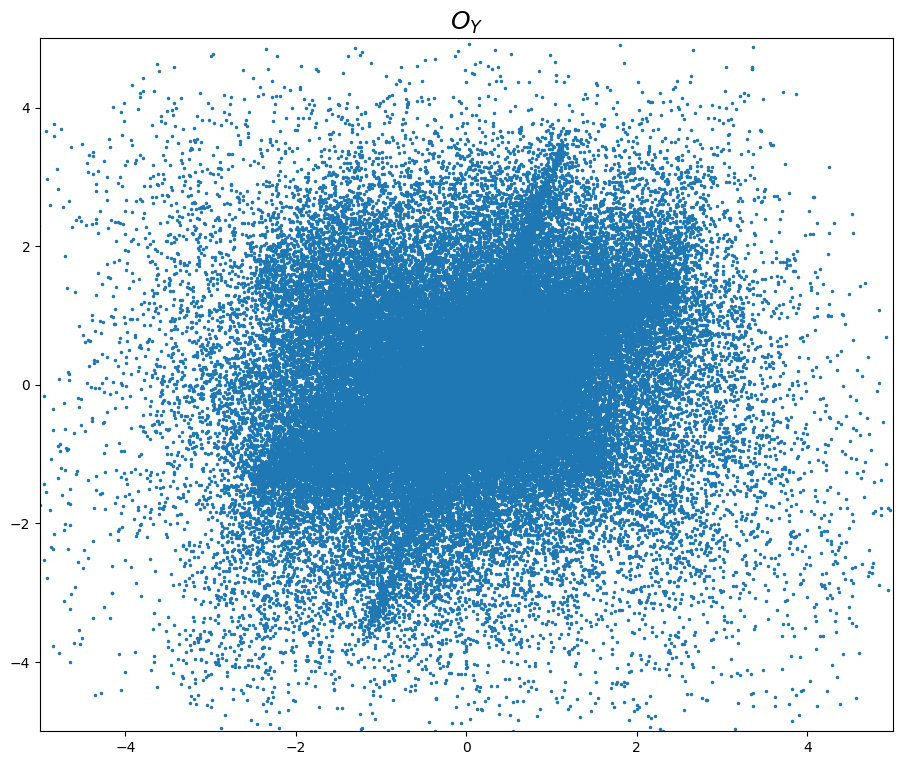
\includegraphics[width=0.5\textwidth]{sources/pc_y.png}} 
    \subfigure[]{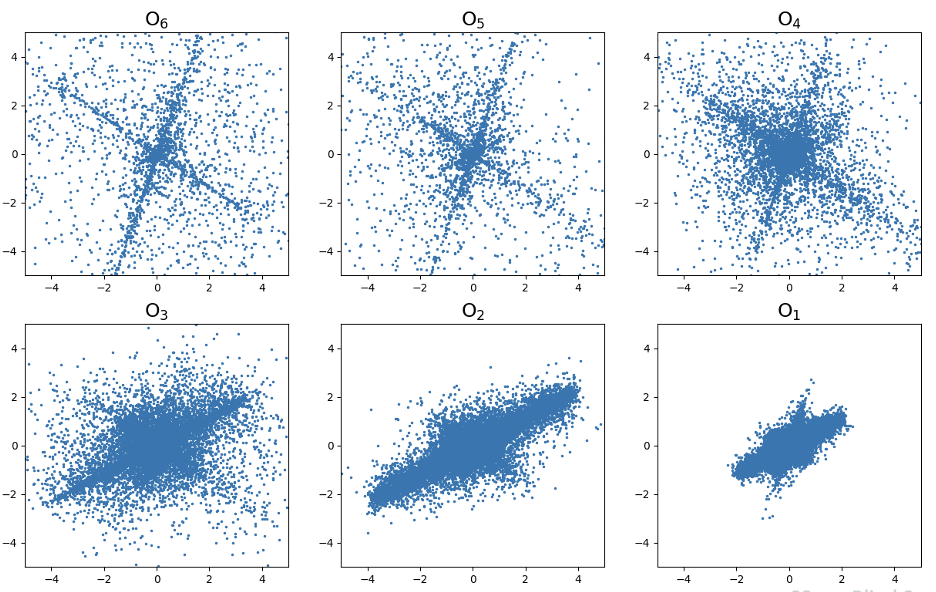
\includegraphics[width=0.5\textwidth]{sources/pc.png}} 
    \subfigure[]{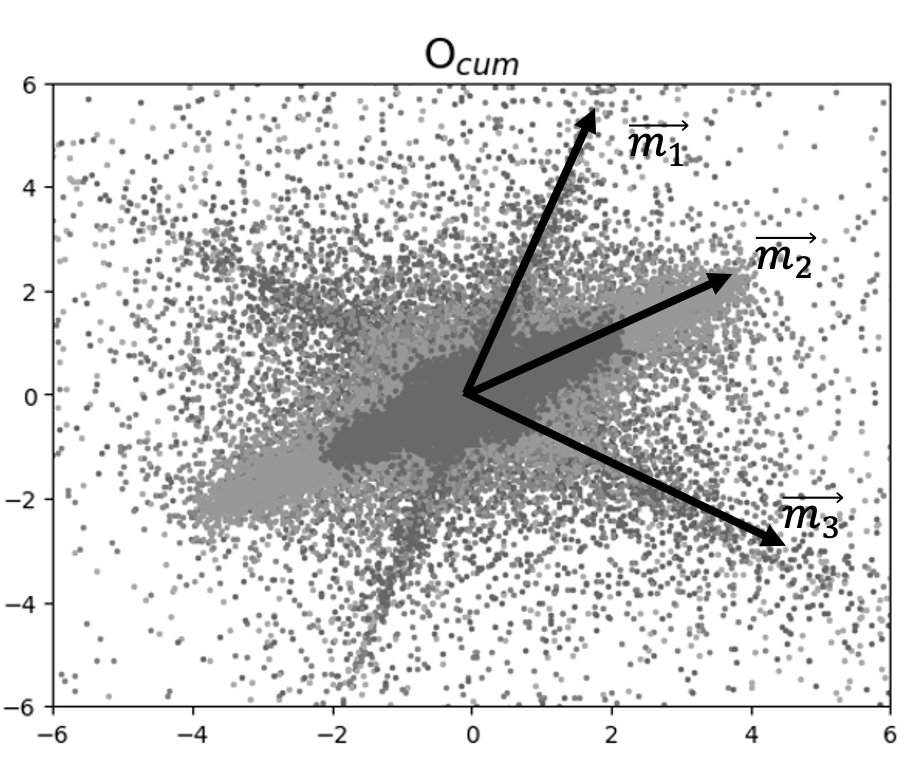
\includegraphics[width=0.4\textwidth]{sources/ocum_angle.png}}
    \caption{\textbf{(a)} Cloud $\{\vec{y}[n]\}_n$ in $ \mathbb{R}^{2}$. \textbf{(b)} Clouds $\{\vec{u}[n_l]\}_{n_l}$ in $ \mathbb{R}^{2}$. \textbf{(c)} Cloud $O_{cum}$.}
    \label{fig:foobar}
\end{figure}
\noindent Yet, there exists a huge number of noisy vectors present at the center of the cloud. 
Thus, we performed a thresholding process that eliminates noisy vectors and keeps the $T=5\%$ vectors of the largest norm. 
\\
\begin{equation}
    \tilde{u} = \{\vec{u} \in \vec{u}[n_l]:\left\lVert \vec{u}\right\rVert \geq T \}
\end{equation}
Then our $\theta$ can be defined by using the trigonometry,
\begin{equation}
    \text{let} \ \; \theta = \arctan(\frac{u_2}{u_1}), \quad \text{where} \; \vec{u} = \binom{u_1}{u_2}, \;\; \vec{u} \in \tilde{u}
\end{equation}
\\
We can construct an angle histogram $H(\theta)$ over all $\theta$. The mixing directions can be identified by detecting local maxima in the histogram $H(\theta)$. Consequently, we can observe that there are $K=3$ sources with directions of $\theta^{*}_1, \; \theta^{*}_2, \text{and} \;\theta^{*}_3$ respectively.


\begin{figure}[H]
\centering
\subfigure[]{
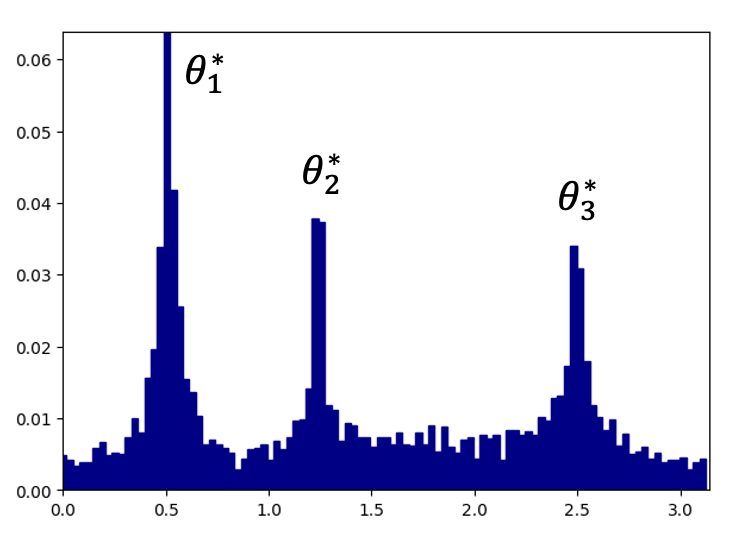
\includegraphics[width=0.5\linewidth]{sources/histogram_angle.png}
}
\caption{ \textbf{(a)} Histogram $H(\theta$) with $\theta^{*}_1, \; \theta^{*}_2, \text{and} \;\theta^{*}_3$ }
\end{figure}

\noindent The estimated directions $\theta^{*}$ are used to estimate the mixing matrix $\hat{M}$. 
\\
\\
Recall that $\vec{u} = \binom{u_1}{u_2}$,
\[
\begin{split}
    \theta^*_k & = \arctan(\frac{u_2}{u_1}), \; \text{for some} \; \vec{u} \in \Tilde{u} \\
    \frac{u_2}{u_1} & = \tan(\theta^*_k) \\
    & = \frac{\sin(\theta^*_k)}{\cos(\theta^*_k)}
\end{split}
\]

\noindent Each $\theta^{*}_1, \; \theta^{*}_2, \text{and} \;\theta^{*}_3$ refers to the mixing directions of each source $s_1[n], s_2[n], \text{and} \; s_3[n]$ respectively. We can then construct our mixing matrix $\hat{M}$ as follows:

\begin{equation}
\hat{M} = \begin{bmatrix}\cos(\theta^*_1)&\cos(\theta^*_2)&\cos(\theta^*_3)\\
\sin(\theta^*_1)&\sin(\theta^*_2)&\sin(\theta^*_3)
\end{bmatrix}
\end{equation} \\




\subsection{Clustering and Signal Reconstruction}

\noindent We now have estimated mixing matrix $\hat{M}$ and wavelet coefficient vectors $\vec{u}[n_l]$. Again, we assume that the coefficients are mostly disjoint and hence the clustering can be performed. For clustering, we used a masking algorithm introduced by Jourjine, Rickard, and Yilmaz \cite{1306640}. The algorithm uses the idea of measuring the cosine similarity, where the inner product of the coefficient vectors and the mixing matrix will be an indicator that tells us which mixing direction a coefficient vector is closest to. \\
\\
Let us represent the estimated mixing matrix as vectors in $\mathbb{R}^{2}$, 
\[
\hat{M} = 
\begin{bmatrix}\cos(\theta^*_1)&\cos(\theta^*_2)&\cos(\theta^*_3)\\
\sin(\theta^*_1)&\sin(\theta^*_2)&\sin(\theta^*_3)
\end{bmatrix}
=
\begin{bmatrix}\vec{m}_1&\vec{m}_2&\vec{m}_3
\end{bmatrix}
\]

\noindent Then coefficients vectors can be clustered with the masking algorithm implemented as follows:
\begin{equation}
    A^*_k=
    \begin{cases} 
    \langle \vec{u}[n_l], \vec{m}_k\rangle, \quad \text{if} \; k = \text{argmax}(\langle \vec{u}[n_l], \vec{m}_{k^{'}}\rangle)_{1 \leq k^{'} \leq 3} \\
    0 \quad otherwise 
   \end{cases}
\end{equation}

\noindent Once the wavelet coefficients are classified, they can be reconstructed back into the original signal by a process called Inverse Discrete Waveform Transform.

\begin{equation}
    \hat{s}_k[n] = IDWT(A^*_k)
\end{equation}

\noindent Here, $\hat{s}_k[n]$ is an estimated sound of the original source $s_k[n]$ multiplied by an arbitrary factor. This is because the normalization process affects the global amplitude and such information is lost after the source separation.



% If the coefficients are mostly disjoint, then the mixing vectors can be identified.
% By our assumption, $c_{k}$ are strictly disjoint.

% \begin{equation}
%     c_{k} \neq 0 \; \Rightarrow \; c_{k^{'}} = 0 \; \ \text{for} \ \; k \neq k^{'}
% \end{equation}

% Which implies that there exists some single $k^*$ where
% \begin{equation}
%     \sum \limits _{{k=1 }}^{K}\vec{m}_{k}c_{k}[n_l] \;
%     = \vec{m}_{k^*}c_{k^*}[n_l], \; k^* \in K
% \end{equation}


\subsection{Results and Conclusion}
\begin{figure}[H]
\centering
\subfigure[]{
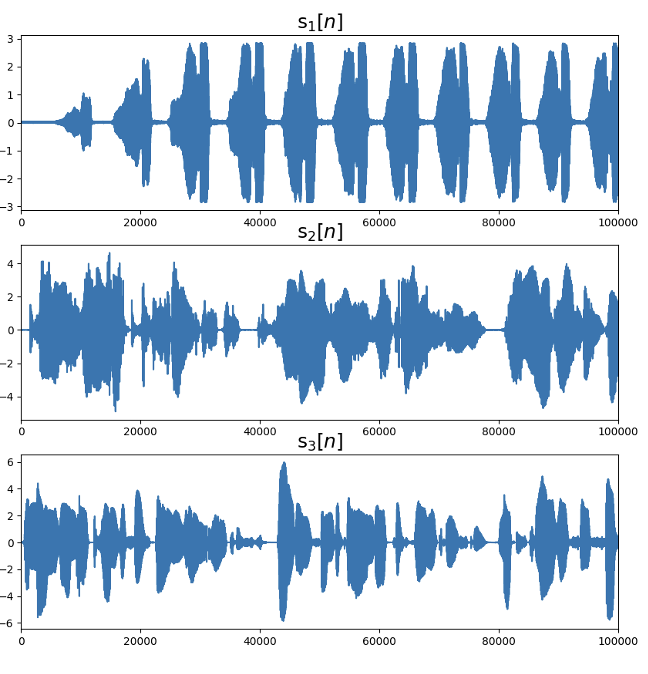
\includegraphics[width=0.43\linewidth]{sources/s.png}
}
\centering
\subfigure[]{
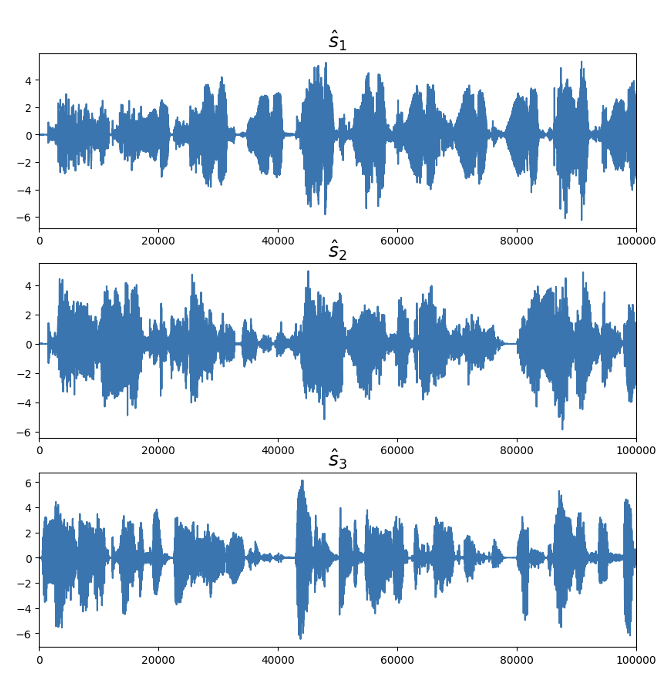
\includegraphics[width=0.45\linewidth]{sources/result.png}
}
\caption{\textbf{(a)} original source signals  \; \textbf{(b)} reconstructed source signals }
\end{figure}

By comparing the original source signals and reconstructed source signals from Figure 5, we can deduce the conclusion that through empirical experiment we have proven that wavelet transform can solve the Blind Source Separation problem given that the sources are sparse in the wavelet domain. \\
\\
\noindent However, it is observable that there exits some noise in reconstructed signals compared to the original signals. This noise is the reconstruction error invoked during the clustering process discussed in section 3.3 of this project, which is unavoidable in our project scope. In a further development, we will try to figure out a way of reducing the reconstruction error by testing various denoising methods such as spatial filtering and wavelet threshold method. 

\pagebreak
\bibliographystyle{ieeetr}
\bibliography{bib}


\end{document}
